\documentclass{beamer}
\usetheme{ConnectivityLab}
\usepackage{times}
\usepackage{graphicx}
\usepackage{verbatim}
\usepackage{outlines}
\usepackage{fancyhdr}
\usepackage{subfigure}
\usepackage{cancel}
\usepackage{bibentry}
\usepackage{varwidth}
\usepackage{etoolbox}
\usepackage{epstopdf}

%%%%%%%%%%%%%%%%%%%%%%%%%%%%%%%%%%%%%%%%%%%%%%%%%%%%%%
%%%%%%%%%%%%%%%%%%%%%%%%%%%%%%%%%%%%%%%%%%%%%%%%%%%%%%

\title {
    progress report 
}
\author {
    Yin-Hong, Hsu
}
\date {
    11 24, 2016
}

%%%%%%%%%%%%%%%%%%%%%%%%%%%%%%%%%%%%%%%%%%%%%%%%%%%%%%
%%%%%%%%%%%%%%%%%%%%%%%%%%%%%%%%%%%%%%%%%%%%%%%%%%%%%%

\begin{document}
\begin{frame}
    \titlepage
\end{frame}

%%%%%%%%%%%%%%%%%%%%%%%%%%%%%%%%%%%%%%%%%%%%%%%%%%%%%%
%%%%%%%%%%%%%%%%%%%%%%%%%%%%%%%%%%%%%%%%%%%%%%%%%%%%%%

\begin{frame}{Outline}
    \tableofcontentsgather
    \tableofcontents
\end{frame}

%%%%%%%%%%%%%%%%%%%%%%%%%%%%%%%%%%%%%%%%%%%%%%%%%%%%%%
%%%%%%%%%%%%%%%%%%%%%%%%%%%%%%%%%%%%%%%%%%%%%%%%%%%%%%
\section{Papers}

%%%%%%%%%%%%%%%%%%%%%%%%%%%%%%%%%%%%%%%%%%%%%%%%%%%%%%
%%%%%%%%%%%%%%%%%%%%%%%%%%%%%%%%%%%%%%%%%%%%%%%%%%%%%%
\begin{frame} {Papers} 
    \begin{itemize}
        \item {Retransmission-based Access Class Barring for RAN overload control in Machine Type Communications}\cite{RACB}
        \item {Efficient LTE Access with Collision Resolution for Massive M2M Communications} \cite{7063635}
        \item {Adaptive RACH Congestion Management to Support M2M Communication in 4G LTE Networks} \cite{6802879}
    \end{itemize}
\end{frame}

\section{brief describe of these paper}
\begin{frame}{Retransmission-based Access Class Barring for RAN overload control in Machine Type Communications}
    \begin{itemize}
            \item {Classify into several groups by the number of retransmission. Each group were assigned a weight which means the proportion of RACH resource they get.}
            \item {The way to control the proportion of RACH resource is dynamic change their ACB factor}
    \end{itemize}
\end{frame}
%%%%%%%%%%%%%%%%%%%%%%%%%%%%%%%%%%%%%%%%%%%%%%%%%%%%%%
%%%%%%%%%%%%%%%%%%%%%%%%%%%%%%%%%%%%%%%%%%%%%%%%%%%%%%

\begin{frame}{Efficient LTE Access with Collision Resolution for Massive M2M Communications}
    \begin{itemize}
            \item {Proposed a collision resolution algorithm. The algorithm use q-ary tree spliting to split the set of avaliable preable}
            \item {Revise MSG4 to make UE next contention attempt use the sub-set of available preamble on dedicate RAO(random access oppo
            rtunity)}
    \end{itemize}
\end{frame}

\begin{frame}{Adaptive RACH Congestion Management to Support M2M Communication in 4G LTE Networks}
    \begin{itemize}
            \item {With several known algorithm for congestion control, and seperate congestion situation in three level.}
            \item {Propose an algorithm ``ARC'', to apply the best congestion control algo to correspond congestion level.}
    \end{itemize}
\end{frame}

%%%%%%%%%%%%%%%%%%%%%%%%%%%%%%%%%%%%%%%%%%%%%%%%%%%%%%
%%%%%%%%%%%%%%%%%%%%%%%%%%%%%%%%%%%%%%%%%%%%%%%%%%%%%%
\section{Classification}
\begin{frame}{{what this paper modify [1]}}
    \begin{itemize}
    \item {MSG3- include number of preamble transmission}
    \item {SIB2- dynamic ACB factor}
    \end{itemize}
\end{frame}
\begin{frame}{{what this paper modify [2]}}
    \begin{itemize}
    \item {MSG4- propose MSG4b to notify the UE about collision and specifying detail of next contention.}
    \end{itemize}
\end{frame}
\begin{frame}{{what this paper modify [3]}}
    \begin{itemize}
    \item {eNB- about congestion control strategy}
    \end{itemize}    
\end{frame}
\begin{frame}{{similarity}}
    \begin{itemize}
    \item {restrict RAP}
    \item {get higher success probability}
    \end{itemize}    
\end{frame}
\begin{frame}{{difference}}
    \begin{itemize}
    \item {[1]- use feedback from MSG3}
    \item {[2]- deal with all collision, get higher delay}
    \item {[3]- use multiple algo to handle different situation}
    \end{itemize}    
\end{frame}

\section{Comparison}
\begin{frame}{Access success probability and delay}
\begin{center}
\begin{tabular}{|c|c|c|c|}
\hline
                         & {[}1{]} & {[}2{]} & {[}3{]} \\ \hline
Access success probility & 2       & 3       & 1       \\ \hline
Access delay             & 1       & 3       & 2       \\ \hline
\end{tabular}
\end{center}
\end{frame}
\begin{frame}{[1] access success probability}
    \begin{figure}[t]
        \centering
        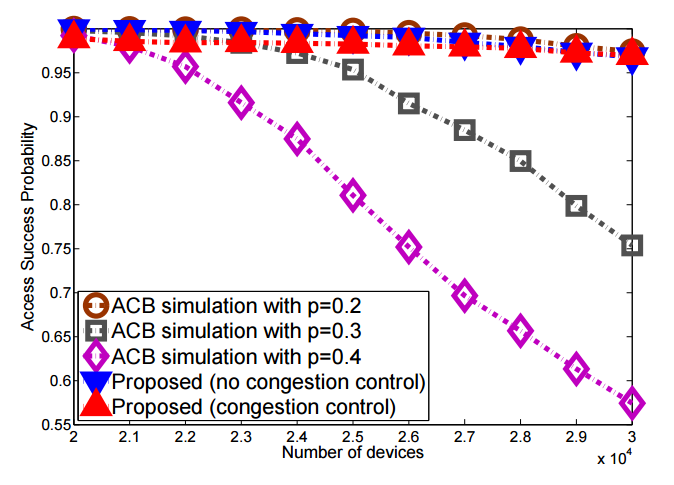
\includegraphics[width=0.8\textwidth]{figures/asp1.png}
        \setbeamerfont{caption}{size=\tiny}
    \end{figure}
\end{frame}
\begin{frame}{[2] outage probability}
    \begin{figure}[t]
        \centering
        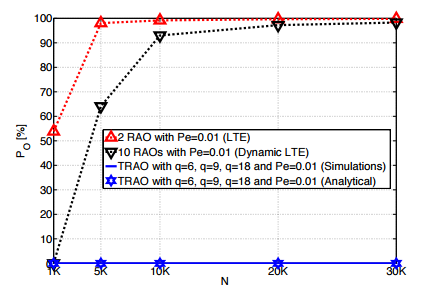
\includegraphics[width=0.8\textwidth]{figures/asp2.png}
        \setbeamerfont{caption}{size=\tiny}
    \end{figure}
\end{frame}
\begin{frame}{[3] access success probability}
    \begin{figure}[t]
        \centering
        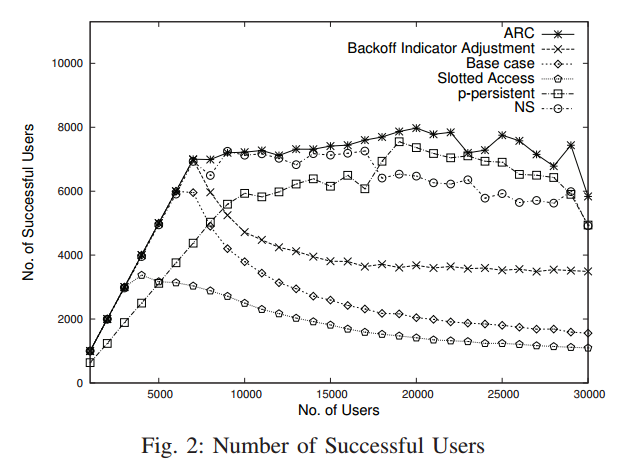
\includegraphics[width=0.8\textwidth]{figures/asp3.png}
        \setbeamerfont{caption}{size=\tiny}
    \end{figure}
\end{frame}
\begin{frame}{[1] access delay}
    \begin{figure}[t]
        \centering
        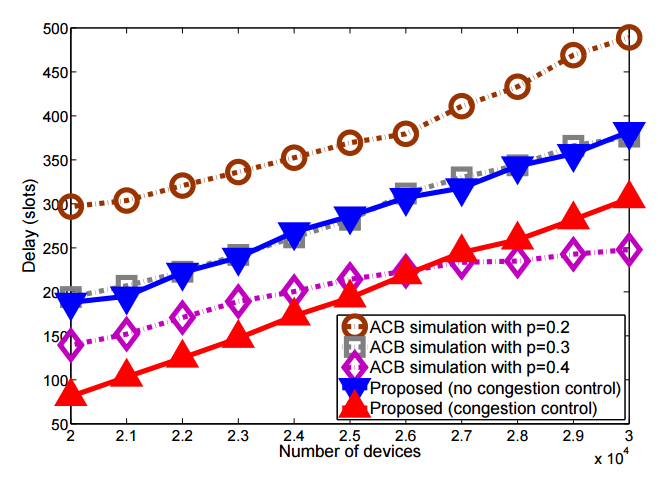
\includegraphics[width=0.8\textwidth]{figures/ad1.png}
        \setbeamerfont{caption}{size=\tiny}
    \end{figure}
\end{frame}
\begin{frame}{[2] access delay}
    \begin{figure}[t]
        \centering
        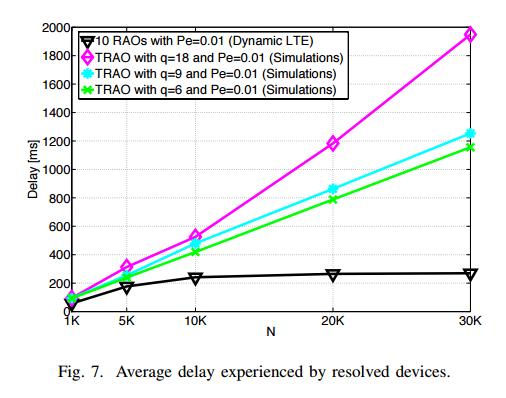
\includegraphics[width=0.8\textwidth]{figures/ad2.png}
        \setbeamerfont{caption}{size=\tiny}
    \end{figure}
\end{frame}
\begin{frame}{[3] access delay}
    \begin{figure}[t]
        \centering
        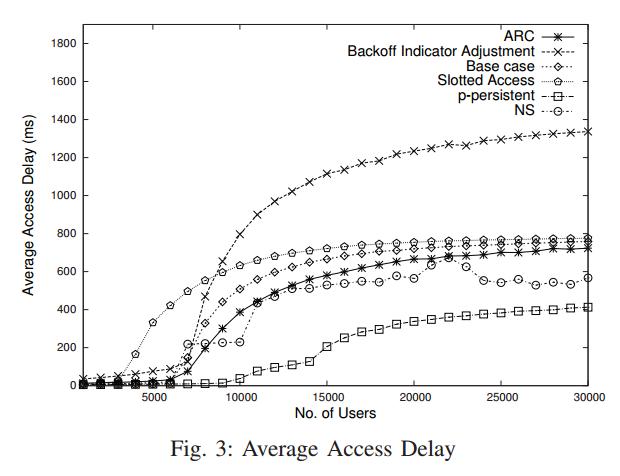
\includegraphics[width=0.8\textwidth]{figures/ad3.png}
        \setbeamerfont{caption}{size=\tiny}
    \end{figure}
\end{frame}
%%%%%%%%%%%%%%%%%%%%%%%%%%%%%%%%%%%%%%%%%%%%%%%%%%%%%%
%%%%%%%%%%%%%%%%%%%%%%%%%%%%%%%%%%%%%%%%%%%%%%%%%%%%%%
\section{References}
\calcreferencespagetotal % Calc your References Page total number
\begin{frame}[allowframebreaks]{References}
    \fontsize{9pt}{13}\selectfont
    \bibliographystyle{IEEEtran}
    \bibliography{IEEEabrv,Citation}
\end{frame}

%%%%%%%%%%%%%%%%%%%%%%%%%%%%%%%%%%%%%%%%%%%%%%%%%%%%%%
%%%%%%%%%%%%%%%%%%%%%%%%%%%%%%%%%%%%%%%%%%%%%%%%%%%%%%
\section{}

\begin{frame}
    \centering
    \Large{Thanks for Your Attentions}
\end{frame}

\end{document}
